
\documentclass[12pt,letterpaper, twoside]{article}


%\usepackage{geometry}
\usepackage{mathrsfs}
\usepackage{epsfig}
\usepackage{helvet}
\usepackage{courier}
\usepackage{amsmath, amssymb, amsthm, amsfonts, graphicx}
\usepackage{url,color}
\usepackage{tabularx}
\usepackage{amssymb}
\usepackage{amsmath}
\usepackage{amsthm}
\usepackage{hyperref}
\usepackage{nicefrac}
\usepackage{graphicx}
\usepackage{epsfig}
\usepackage[nottoc]{tocbibind}


\usepackage{tabu}
\usepackage{algorithm}
\usepackage[noend]{algpseudocode}
\usepackage{wrapfig}
\usepackage{empheq}
\usepackage{ragged2e}
\usepackage{multicol}
\usepackage{mathtools}
\usepackage{pstricks-add, auto-pst-pdf}
\usepackage{tikz}
\usepackage{textcomp}
\usetikzlibrary{positioning,chains,fit,shapes,calc}

\frenchspacing
%\newtheorem{theorem}{Theorem}
\newtheorem{note}{Note}
\newtheorem{lemma}{Lemma}
\newtheorem{prop}{Proposition}
\newtheorem{theorem}{Theorem}
\newtheorem{definition}{Definition}
\theoremstyle{definition}
\newtheorem{exmp}{Example}[section]

\usepackage{tikz}
\usetikzlibrary{calc}
\usepackage{caption}
\setlength{\topmargin}{ 0.1in}
\setlength{\columnsep}{2.0pc}
\setlength{\headheight}{0.0in} \setlength{\headsep}{0.0in}
\setlength{\oddsidemargin}{.15in} \setlength{\parindent}{1pc}
\setlength{\evensidemargin}{.15in} \setlength{\parindent}{1pc}
\setlength{\parsep}{15pt}
\textheight 9.0in \textwidth 6.0in
\graphicspath{{./images/}}
% \newcommand{\hr}{\noindent\rule{\textwidth}{.35mm}\vspace{8pt}}% 




\begin{document}


\begin{table}[!h]
\centering
%\resizebox{\textwidth}{!}{
\begin{tabularx}{\textwidth}{|Xll|}
\hline
& &\\
Probabilistic Graphical Models &  Date: & \emph{12 April 2020}\\
 & &\\
Instructor: \emph{Girish Varma} & Team Members: & {Chaitanya Kharyal , Tanmay Kumar Sinha} \\ 
 \hline

\end{tabularx}
%}
\end{table}

\begin{center}
\begin{LARGE}
Quasi-Monte Carlo Markov Chain Methods
\end{LARGE}
\end{center}

\tableofcontents

\section{Introduction}
In this project, we attempt to explain the concept of Quasi-Monte Carlo Markov Chain methods. We will begin by a motivating example, and then illustrate how the Quasi-Monte Carlo methods are useful over the traditional Monte Carlo methods. This is followed by a few technical definitions which help in the analysis of such algorithms, and then the quasi Monte Carlo methods are introduced and we introduce some theorems that show why the Quasi Monte Carlo methods work better in some situations. After this, an introduction to the Quasi Monte Carlo Markov Chain algorithm is given, and a Quasi-Monte Carlo Metropolis Algorithm is shown.


The main idea behind these methods is to use \emph{quasi-random}
 numbers, instead of truly random or pseudo-random numbers, in the randomized algorithms. Quasi-random numbers are not random, in the sense that they are not sampled but are deterministically generated. These have an advantage over pure random numbers as they "cover" the domain of interest, in the sense that is made precise later, more quickly and evenly. The measure of this "cover" can be defined using the concept of \emph{discrepancy}, and the sequences of numbers considered to be quasi-random are those sequences which have a low discrepancy.

The below given image shows 10 points sampled randomly, and 10 points generated according to a low discrepancy sequence called the van der Corput sequence. Notice the more equidistributed nature of the van der Corput sequence.

\begin{figure}[h]
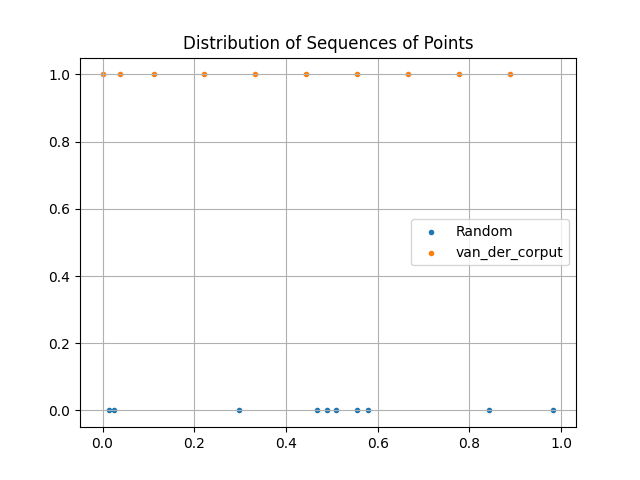
\includegraphics[width=8cm]{images/van_der_corput.png}
\centering
 \end{figure}
 
 
 \section{Motivation: Estimating Integrals}
The main motivating example for the method is the problem of calculating the value of a definite integral i.e. calculating 

$$
I = \int_{0}^{1} f(x)dx
$$ where $f:[0,1] \to \mathbb{R}$ is a real valued function for which the integral is defined i.e which is integrable in $[0,1]$.
Many problems can be reduced to this problem(or its more generalized variant, where the function is a multivariable scalar function over the unit cube of dimension d, and the integration is carried out over the entire cube), such as calculating expectations of random variables, carrying out simulations, etc. For example, consider the problem of finding $\mathbb{E}[f]$ i.e the expectation of a function of a random variable $x$, where domain of x is $[a,b]$. If $x \sim p$, where $p$ is a distribution on $[a,b]$, then we may write  

$$
\mathbb{E}[f] = \int_{a}^{b}f(x)p(x)dx
$$ 
Thus, we have reduced this problem to finding a definite integral.

The simplest method of calculating the definite integral is to use what is called the rectangle rule - you divide the interval into $N$ equally spaced points, and approximate the integral as
$I_N = \frac{1}{N}\sum_{i=1}^{N}f(\frac{i}{N})$. From the definition of the integral, we have 

$$
\lim_{N \to \infty} I_N = I
$$

Essentially, this method is one where we use $x_i = i/N$ as our sequence.

This method may work well for one dimensional integrals, but the complexity of the integral rises rapidly with the increase in dimensions - in general, to divide the $s$-dimensional unit cube, you would need $\mathcal{O}(N^s)$ points. This becomes difficult for high dimensional integrals. The problem can be circumvented by using randomized techniques, such as the Monte Carlo method.

\subsection{Monte Carlo Method}

Consider our original problem i.e. of finding 

$$
I = \int_{0}^{1}f(x)dx
$$

The traditional Monte Carlo \cite{owenReport}\cite{kuoReport} method works by sampling $x_1,x_2,\ldots,x_N$ uniformly from $[0,1]$, and approximating $I$ as $I_N$, where

\begin{equation}
    I_N = \frac{1}{N}\sum_{i=1}^{N}f(x_i)
\end{equation}


Then, the error, $\epsilon_N = |I - I_N|$, is a random variable. Using the  strong law of large numbers, we can derive that

$$
Pr[\lim_{n \to \infty} \epsilon_n = 0] = 1
$$ 

Also, using the Central Limit theorem, we may say that the root mean square error in the error is of the order $\frac{1}{\sqrt{N}}$ i.e. the RMSE error is $\mathcal{O}(\frac{1}{\sqrt{N}})$.

This technique is useful in particular for high dimensional integrals, where sampling points in $s$-dimensional space may be easier. Additionally, you can keep sampling points, while also using all the previously generated random points, to get your desired level of accuracy - this was an issue if we used the rectangle rule, where you would need to recompute all the previous points to again calculate the integral, if you needed more accuracy.

Also, when calculating expectations, the Monte Carlo method offers us some more advantages. For simplicity, let us say $X$ is a random
variable over some domain $D$,distributed according to some probability distribution $P$, and $f:D \to \mathbb{R}$ is a function. Then, to calculate $\mathbb{E}[f(X)]$, we may use the
integration approach - 

$$
\mathbb{E}f = \int_D f(x)P(x)dx
$$

We can approximate it using the traditional Monte Carlo approach by taking a sequence of uniformly distributed random numbers $\{x_i\}$in $D$, and calculating $$
I_N = \frac{1}{N}\sum_{i=1}f(x_i)P(x_i)
$$

However, if calculating $P(x_i)$ is difficult, or we do not know $P$ explicitly, we may use a slightly altered Monte Carlo method - instead of sampling  $\{x_i\}$ uniformly from $D$, we may sample $\{x_i\}$ directly from $P$. Then, our $P(x_i)$ term would be implicit in our sampling, and we could approximate the expectation by

$$
I_N = \frac{1}{N} \sum_{x_i \sim P} f(x_i)
$$

The above is a powerful method and is very useful when we may not explicitly know the underlying distribution, but sampling from that distribution is possible. It becomes even more powerful as we may now use our randomized methods in our graphical models such as Bayesian networks and Markov Networks, provided they are easy to sample from.

\section{Some Definitions and Results}

\subsection{Discrepancy}

\begin{definition}[Discrepancy(in one Dimension)]
Let {$s_i$} be a sequence in $\mathbb{R}$, and $[a,b] \subsetneq \mathbb{R}$. Then, the \emph{discrepancy} of the sequence with respect to $[a,b]$ is defined as


$$
D_N = \sup_{a \leq c \leq d \leq b} \left| \frac{\mid \{s_1,s_2,\ldots s_N\} \cap [c,d]\mid}{N} - \frac{d - c}{b - a} \right| 
$$
\end{definition}
Informally speaking, the discrepancy measures the proportion of points that fall into the region $[a,b]$. A sequence will have low discrepancy if the proportion of points that fall into the set is comparable to the size of the set (which would be the case for a uniformly distributed sequence).

To generalize the definition given above to a general, multidimensional case, multiple definitions are possible. However, for our purposes, the below given definition is sufficient. 

\begin{definition}[Discrepancy(general definition)]
Let $\{x_1,x_2,\ldots x_N\}$ be a sequence in $\mathbb{R}^s$, and $I^s = [0,1] \times [0,1] \times \ldots \times [0,1]$ be the $s$-dimensional hypercube. Then, the discrepancy of the sequence w.r.t the set $I^s$ is defined as 

$$
D_N(x_1,x_2,\ldots,x_N) = \sup_{B \in J} \left| \frac{A(B)}{N} - |B|\right|
$$where :-

$J$ is the set of all $s$-dimensional intervals of $I^s$, i.e. 
$$
J = \left\{ \prod_{i=1}^{s} [a_i,b_i), where 0 \leq a_i \leq b_i \leq b_i \right\}
$$

$A(B)$ is the number of point of $\{x_1,x_2 \ldots ,x_N\}$ that lie in B i.e
$ A(B) = \left| \{x_1,x_2 \ldots ,x_N\} \cap B\right| $

$|B|$ is the size of B i.e. the (hyper)volume of B.
\end{definition}

One additional definition we need before proceeding further is the definition of \emph{Star discrepancy}. To define star discrepancy, we replace $J$ by $J^*$ in the definition of discrepancy, where $J^*$ now includes only closed intervals instead of half-open half-closed intervals. Formally,  
$$
J^* = \left\{ \prod_{i=1}^{s} [a_i,b_i], where 0 \leq a_i \leq b_i \leq b_i \right\}
$$

Thus, we have the definition of star discrepancy:-

\begin{definition}[Star Discrepancy] \cite{kokshmaWikipedia}
Let $\{x_1,x_2,\ldots x_N\}$ be a sequence in $\mathbb{R}^s$, and $I^s = [0,1] \times [0,1] \times \ldots \times [0,1]$ be the $s$-dimensional hypercube. Then, the star discrepancy of the sequence w.r.t the set $I^s$ is defined as 

$$
D_N^*(x_1,x_2,\ldots,x_N) = \sup_{B \in J^*} \left| \frac{A(B)}{N} - |B|\right|
$$, where $J^*$ is as defined above.
\end{definition}
\subsection{Koksma-Hlawka Inequality}
\begin{theorem}[Koksma-Hlawka Inequality] \cite{owenReport}\cite{kokshmaWikipedia}
Let $f:I^s \to \mathbb{R}$ be a multiriable function such that $f$ has $bouded$ $variation$ $V(f)$ on $I^s$. Then, for any $\{x_1,x_2,\ldots ,x_N\}$ in $I^s$, we have

$$
\left|\frac{1}{N}\sum_{i=1}^{N} f(x_i) - \int_{I^s}f(x)dx\right| \leq V(f) D_N^*(x_1,x_2,\ldots,x_N)
$$
\end{theorem}

The term $V(f)$ here is the total variation, a technical term that is not of much concern to us, other than the fact that it is a constant that depends only on $f$. The total variation of a 1D function is a measure of the 1D arc length of the parametric curve $(t,f(t)$, where $t \in [0,1]$. The total variation in multiple dimensions is a similar concept. We require that the function have \emph{bounded variation} i.e. the total variation be less than infinity.

The Koksma-Hlawka inequality is a very important result, as it allows us to measure the error in our approximated quantity only in terms of the discrepancy of the used sequence of numbers. Thus, if we can form sequences which are of low discrepancy, then we can reduce the error substantially. The construction of one such sequence is given below.

\subsection{van der Corput Sequence}

The van der Corput sequence \cite{kokshmaWikipedia}\cite{VanDerWiki} is a simple example of a 1D low discrepancy sequence. It is important because we may use this sequence to generate many other high dimensional low discrepancy sequences, such as the Halton sequence. 

Informally, the $n^{th}$van der Corput sequence with base $b$ is generated by flipping the exponent in the base $b$ expansion of $n$. More formally, if 

$$
n = \sum_{k=0}^{L-1}d_n(k) b^k,
$$ where $d_n(k)$ is the $k^{th}$ "digit" in the $b$-ary expansion of n, then the $n^{th}$ element of the van der Corput sequence in base $b$ is given by 

$$
g_b(n) = \sum_{k=0}^{L-1}d_n(k)b^{-k-1} = \sum_{k=0}^{L-1}\frac{d_n(k)}{b^{k+1}}
$$

\begin{theorem}[Low Discrepancy of the van der Corput Sequence]
Let $\{g_b(1),g_b(2), \ldots , g_b(N)\}$ be the van der Corput sequence for some base $b$. Then $\exists C(b) \in \mathbb{R}$ such that

$$
D_N^*(\{g_b(1),g_b(2), \ldots , g_b(N)\}) \leq C(b) \frac{\log N}{N}
$$
\end{theorem}
A simple corollary of the above theorem is that, if we use a van der Corput sequence to evaluate an integral, then the error of that integral is $\mathcal{O}(\frac{\log N}{N})$

\section{Quasi-Monte Carlo Methods}

\subsection{Quasi Monte Carlo method}
The Quasi Monte Carlo Method \cite{owenReport}\cite{kuoReport}\cite{qmcWikipedia} also takes the same form as the traditional Monte Carlo Method, (As represented by equation \textbf{(1)}) the difference is that, instead of sampling uniformly distributed random numbers, we use deterministically generated quasi random numbers (for example, van der Corput sequence). In this way we get the points which are more uniformly distributed than the random points. These points, then, give us more understanding of the function we are trying to integrate, and thus results in faster convergence.

Then, the approximation error of the QMC is bounded by a term (given by Koksma–Hlawka inequality) proportional to the \textit{discrepancy} ($D$) of the quasi random points and the \textit{variation} ($V$) of the integrand $f$ (in Hardy and Krause sense). Formally,

\begin{equation*}
    |I(f) - Q(f)| \;=\;  |\frac{1}{N}\sum_{i=1}^{N}f(x_i) - \int_{\overline{I}_s}f(x)dx| \; \leq \; D(x_0, x_1, \dots, x_{N-1})V(f) 
\end{equation*}

where, $\overline{I}_s$ is a unit cube of $s$ dimension. ie. $\overline{I}_s = [0,1] \times \dots \times [0,1]$

Thus, we can show that the error in the value of our estimate depends only on the discrepancy of the sequence of points. We can construct sequences which have very low discrepancies, of order $\mathcal{O}(\frac{\log(N)^s}{N})$, which is much better than the RMSE error of the traditional Monte Carlo method for large $N$ and small $s$.

Note that the points for QMC are generated to be more uniform than random  numbers. The degree of uniformity is typically quantified as the distance between discrete uniform distribution on $x_i$ and continuous uniform distribution on $[0,1]^{s}$ and this is the $D$ used in the above equation. One such measure of distance is Star Discrepancy. For defining Star Discrepancy, let us first define a function called Local Discrepancy function at a point $a$,

\begin{equation*}
    \delta(a) = \text{Vol}([0,a]) - \frac{1}{N}\sum_{i=1}^{N} 1_{x_i \in [0,a]}
\end{equation*}
Here, Vol$([0,a])$ is the volume of $s$ dimensional box with opposite corners at $0$ and $a$.

Now, we can define the star discrepancy, specific to this case, as,

\begin{equation*}
    D_n^*(x_1, \dots, x_n) \;=\; \underset{a\in[0,1]^s}{\text{max}}|\delta(a)|
\end{equation*}


\subsection{Randomized Quasi Monte Carlo Method}
The bound given by Koksma-Hlawka inequality is very poorly suited to estimate error because it contains discrepancy term $D_n^*$ which is very hard to compute and the variance $V$ is ordinarily harder to find. Therefore, we use a hybrid of MC and QMC, Randomized Quasi Monte Carlo method.

RQMC \cite{owenReport}\cite{qmcWikipedia}\cite{owenReport2} randomizes the QMC points in such a way that for the RQMC point set $P_N = \{x_0,\dots,x_{N-1}\}$:

\begin{itemize}
    \item Each $x_i$ is uniformly distributed over $(0,1)^s$.
    \item $P_N$ as a whole is a low discrepancy set.
\end{itemize}

Thus, QMC is reduced to variance reduction method. The RQMC estimator,
\begin{equation*}
    I(f) = \frac{1}{N}(\sum_{i = 0}^{N-1}f(U_i))
\end{equation*}
\begin{equation*}
    \implies \text{Var}(I(f)) = \frac{Var[f(U)]}{N} + \frac{2}{N^2}\sum_{i<j}\text{Cov}[f(U_i)f(U_j)]
\end{equation*}

Now, the first term in the above equation is always positive, therefore if we want to minimise the variance, we will have to make the second term as negative as possible, by inducing pairwise negative covariance. Well known ways of creating such negative correlation include antithetic variates, Latin hypercube sampling (LHS), and stratification.

\newpage

We have implemented one such RQMC algorithm using LHS \cite{LHSWiki}. We have tried to estimate the area under $y = x^2$ curve. The variance plots of traditional MC and RQMC are shown in the figure below

\begin{figure}[h]
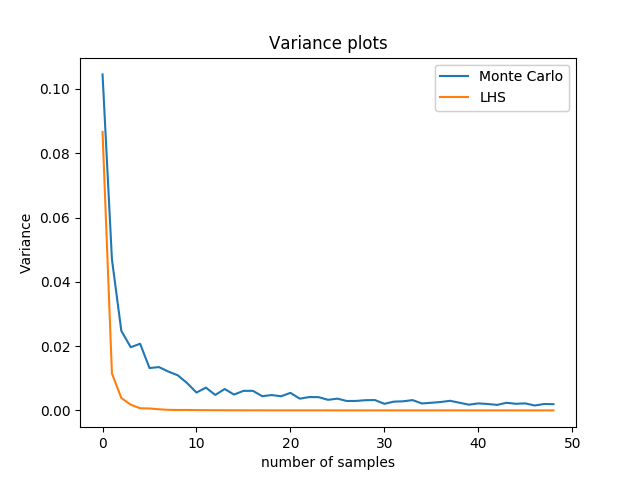
\includegraphics[width=8cm]{images/variance_LHS_vs_MC.png}
\centering
\end{figure}
 
The figure clearly shows the variance of RQMC using LHS is always less than traditional MC.


\section{Markov Chain Monte Carlo}
In this section, we describe how we can apply concepts of QMC to get at a Metropolis-Hastings - like algorithm \cite{owenReport}\cite{owenBook}\cite{cryptoExample}\cite{MCMCslides}. The main reference for this section is \cite{owenReport}. We first describe the Metropolis-Hastings algorithm in brief, and introduce some of the notation to be used. Then, we introduce a Metropolis-Hastings algorithm that uses a special class of quasi-random sequences \cite{owenReport}\cite{owenReport2}, called \emph{completely uniformly distributed} sequences. Then, certain results regarding the above algorithm are discussed.

\subsection{Metropolis-Hastings}
The main problem which the Metropolis-Hastings algorithm tries to tackle is the problem of sampling from some probability distribution, say $P$. Sampling becomes difficult when we are dealing with large graphical models, such as Markov chains and Bayesian networks. In these cases, randomized algorithms, such as the Monte-Carlo methods are useful as they allow us to sample from the distribution quickly and more efficiently. 

In the Metropolis-Hastings algorithm, there are two steps - one is the \emph{proposal} step, the other is the \emph{acceptance} step. In the proposal step, if we are at the $i^{th}$ iteration, then we specify a distribution $p_i$, such that $p_i(x \to y)$ denotes the probability of proposing to move to $y$, given that the current state is $x$. Then, in the acceptance step, we calculate the acceptance probability as 

$$
A(x \to y) = min \left\{ 1,\frac{P(y)p_i(y \to x)}{P(x)p_i(x \to y)}\right\}
$$

Let us say that, at the $i^{th}$ iteration, we are at the state $x_i$. Then, to see what are next state is, we pick a random state $y_i$, generate a random number $u$ sampled uniformly from $[0,1]$ and then, if $u \leq A(x_i \to y_i)$, we move to $y_i$ else we stay at $x_i$. Therefore, we have the following update rule:-

$$
Pick \ u \in_r [0,1]
$$
$$
x_{i+1} =  \begin{cases} 
    y_i & u \leq A(x_i \to y_i) \\
    x_i & otherwise
    \end{cases}
$$

We say that the Markov Chain is homogenous if $p_i$ does not depend on $i$ i.e. is the same in all iterations.

Let $\Omega = \{\omega_1,\omega_2,\ldots \omega_K\}$ be the state space. Then, for such a finite, discrete state space, the MCMC algorithm can also be written in the matrix form, by maintaining a belief vector $v \in \mathbb{R}^K$, such that $v_i$ denotes probability of being in $\omega_i$. Then, after each update, we can write the new belief vector as $v_{i+1} = M_iv_i$, where $M_i$ is a matrix that can be obtained, given $A,p$ and $p_i$. Assuming that the Markov chain is ergodic i.e. aperiodic and the graph of the chain is fully connected, we can prove that the MCMC algorithm tends to the steady state distribution of the Markov Chain i.e. our belief vector converges to a vector $v$ such that $v_i = p(w_i)$.

If we naively try to extend the Metropolis-Hastings algorithm to a quasi-random case i.e. we start sampling $u$ from a quasi-random sequence, then it is observed that the algorithm fails. For example, \cite{owenReport} cites certain cases where using the simple van der Corput sequence tends to not sample the Markov Chain nicely. We need a more stronger type of sequence, and we need to tweak the algorithm a bit, so that it works nicely. 

\subsection{Completely Uniformly Distributed Sequences}
\begin{definition}[Completely Uniformly Distributed]\cite{owenReport}
The sequence $\{u_i\}\in[0,1]$  is said to be completely uniformly distributed (CUD) if $\forall d \geq 1$, the points $z_i = (u_i,u_{i+1},\ldots u_{i+d-1}) \in [0,1]^d$ satisfy

$$
\lim_{N \to \infty} D_N^*(z_1,z_2,\ldots,z_N) = 0
$$

\end{definition}

Note that the $z_i$ defined above forms a bunch of intersecting $d$-tuples. For the algorithm which we will implement, we would need non-intersecting tuples. We have the following lemma \cite{lemma1Book} which helps.

\begin{lemma}
If the sequence ${u_i}$ is a CUD, and $z_i = (u_{di-d},\ldots u_{d_i})$, then 

$$
\lim_{N \to \infty} D_N^*(z_1,\ldots,z_N) = 0
$$
\end{lemma}
Completely uniformly distributed sequences are a more specific type of sequence than low discrepancy sequences. Several ways to construct such sequences exist, but are not discussed here. In practice, some approximations are used to get CUDs from sequences of linear congruential generators, which are a type of pseudorandom number generators such that the $n^{th}$ element is given by the following recurrence:-
$$
X_{n} = (aX_{n-1} + c) \ mod \ m
$$ where $m,c$ and $X_0$ are parameters.


\subsection{Quasi Markov Chain Monte Carlo Algorithm}
We try to extend our idea of normal Metropolis Markov Chain algorithm. Instead of using one random number to generate a transition, we use $d$ numbers, where $1\leq d< \infty$. We assume the proposed transition $y_{i+1}$ can be written as a function $\Psi_{i}$ of $x_i$ and $d-1$ uniformly distributed random variables. Once the transition is decided, one random variable is used to accept or reject the transition. Formally,

\begin{equation*}
    y_{i+1} = \Psi(x_i, u_{di+1}, \dots, u_{di+d+1}) \; \; \; \;\;\;\; \forall i \in \{0,\dots, n-1\}
\end{equation*}

\begin{equation*}
    x_{i+1} =
     \begin{cases}
        y_{i+1}       & \quad \text{if } \; u_{di+d} \leq A_i(x_i \to y_{i+1})\\
        x_i  & \quad \text{otherwise,} 
    \end{cases}
\end{equation*}
The first equation, here, shows generating a transition while the second equation shows the acceptance rejection decision for a state $x_i \in \Omega$ (same as used in Metropolis-Hastings) and random points $u_j \in [0,1]$. 

Now, consider a finite state space Markov chain. Then, our estimated probability distribution i.e the probability of being in some state $\omega$ in the $n^{th}$ iteration, can be written as a function $\hat{p}_n : \Omega \to [0,1]$ defined by 

$$
\hat{p}_n(\omega) = \frac{1}{n}\sum_{i=1}^{n} I[x_i = \omega]
$$ where $x_i$ is the state at $i^{th}$ iteration, and $I$ is the indicator function which is 1 if $x_i=\omega$ and 0 otherwise.

For our algorithm to work optimally, we require that our estimated probability distribution converge to the actual probability distribution that we are trying to sample from. Formally, we require that
$$
\hat{p}_n(\omega) \to P(\omega) \ \forall \omega \in \Omega 
$$ or 
$$
\lim_{n \to \infty} \hat{p}_n(\omega) = P(\omega) \ \forall \omega \in \Omega 
$$ 

The above is an equivalent of the law of large numbers for quasi-random sequences. The law of large numbers is what allows us to use Monte Carlo methods to estimate values, and thus, the above condition will allow us to use quasi-Monte Carlo methods to do the same tasks. We say that the above ensures \emph{consistency} of the algorithm. 
To guarantee that the algorithm remains consistent, we want that the above law of large number holds. We would like to know the sufficient conditions under which this holds. There are some known results which guarantee this. Specifically, we require two conditions - one of \emph{regular proposals}, and the other condition is the existence of a \emph{home state}.

\begin{definition}[Regular Proposal]
The proposals are said to be regular if 
$$
\forall i \geq 0 \; \forall k \;\in \Omega \; \forall l \; \in \Omega, \;\;\text{the set}
$$

$$
S_{i,k \to l} = \left\{ (u_{di+1},\ldots,u_{di+d-1})|y_{i+1} = \omega_l,x_i = \omega_k  \right\}
$$
has a (d-1)-Dimensional boundary of (d-1) dimensional volume 0.
\end{definition}

The above holds for almost all $\Psi$ functions used. The second condition, existence of a home state, basically means a state that can be visited by the algorithm in any stage. More specifically, that for a fixed box $\mathbb{B}$, if our pseudo random numbers are generated in that box, then we always end up in the home state.

\begin{definition}[Home State]
A state $\omega\in \Omega$ is said to be a homestate if $\exists \mathbb{B} \subset [0,1]^d$ such that

$$
(u_{di+1},\ldots,u_{di+d-1}) \in \mathbb{B} \implies x_{i+1} = \omega
$$
\end{definition}

We have the following theorem(the proof is omitted as it quite complicated).

\begin{theorem}
Suppose that, in the Quasi Monte Carlo Markov Chain algorithm given above, the proposals are all regular proposals, the sequence $\{u_i\}$ is a completely uniformly distributed sequence, and $\Omega$ contains a home state with box $\mathbb{B}$. Then, the following limit holds:-

$$
\lim_{n \to \infty} \hat{p}_n(\omega) = P(\omega) \ \forall \omega \in \Omega 
$$ 

\end{theorem}

The conditions given in the above theorem are not very hard to ensure. Thus, in practise, our algorithm is consistent. \cite{owenReport} details some illustrations and simulations, and observes that " QMC-MCMC hybrid consistently had smaller variance than MCMC, sometimes by a small amount, sometimes by a factor of hundreds".

\section{Implementations and Simulations}
As part of the project, to demonstrate why the quasi Monte Carlo method works better in practised, we wrote some Python scripts to demonstrate the advantages of such a method.

\newpage

First, we wrote a script to generate van der Corput and Halton sequences. They were used to demonstrate how we can easily generate low discrepancy sequences and show how they were more evenly ordered as compared to pseudorandom numbers. The image attached below shows a Halton sequence(with bases 2 and 3) of length 100 plotted alongside a pseudo-random sequence of length 100.

\begin{figure}[h]
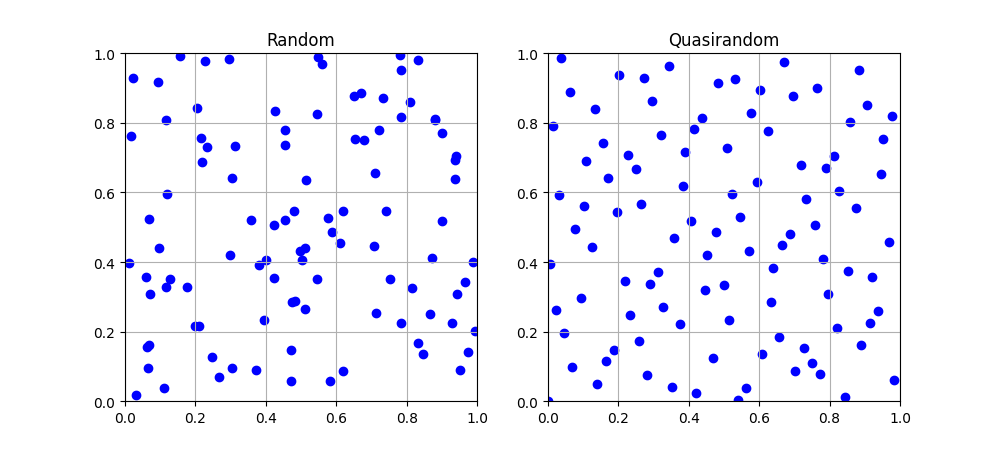
\includegraphics[width=12cm]{images/halton_sequence.png}
\centering
 \end{figure}

Next, we used these sequences to write a simple program that would evaluate $\int_{0}^{1}x \sin{x}dx$, and the error was compared by calculating the definite integral manually and inputting known values. The plot for the errors compared to the number of samples taken is shown below:-

\begin{figure}[h]
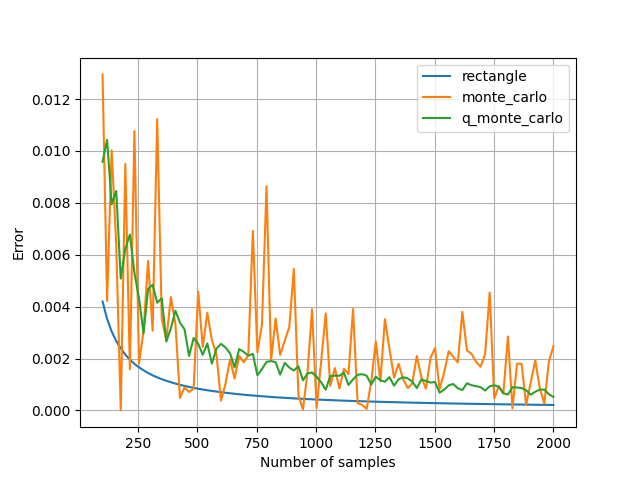
\includegraphics[width=12cm]{images/xsinx.png}
\centering
 \end{figure}

Note the erratic behaviour in the error in the Monte Carlo solution. This is because the Monte Carlo method is a random method. This behaviour can be mitigated partially by running the method N times, and taking the average. Also, note how the Quasi Monte Carlo performs on average better than the Monte Carlo method. However, it loses out to the rectangle method.

But this is only because this integral is a 1D integral. To actually see the power of the quasi Monte Carlo method, we would need to look at a multiple integral. So, we wrote a script to compute the area of an $s$-dimensional hypersphere of radius 1, and compare it to the known value(we know a general formula to calculate the volume of an $s$-D hypersphere. We used the values of s between 3 and 10. We can represent the volume as 

$$V = 2^s \times \int_{I^s}f(x)dx$$ where 

$$
f(x) =  \begin{cases} 
    1 & ||x|| \leq 1 \\
    0 & otherwise
    \end{cases}
$$

Integrating this using the rectangular rule would be difficult in higher dimensions as we would need to divide the interval into many points. Thus, the quasi Monte Carlo method here performs better than the rectangle rule as it takes much less time to compute the random points. 
\medskip


\bibliographystyle{unsrt}
\bibliography{ref}



\end{document}